\documentclass[12pt]{article}
\usepackage{pslatex,multicol,verbatim,wrapfig,pdfpages,url}

\title{Parallel Molecular Dynamics with a Time-Reversible Nos\'{e}-Hoover Thermostat on CPUs and GPUs}
%\subtitle{APC 523}

\author{Nathan Mahynski \and George A. Khoury \and Carmeline Dsilva}


\begin{document}

\maketitle

\section{Introduction}

Due to the dramatic increase in computing power over the last thirty years, molecular dynamics (MD) simulations have become a remarkably fruitful tool for scientific discovery and engineering exploration \cite{Karplus2002,Levitt2001}.
%
These simulations allow us to screen potential drug compounds \cite{Jorgensen2004}, explore protein folding dynamics \cite{Duan1998,Shaw2010,Piana2013,Lindorff-Larsen2011}, study \cite{Boero1998} and develop \cite{Zipoli2010} new catalysts, and explore extreme conditions (temperatures and pressures) that are experimentally inconvenient all without running expensive and time-consuming experiments in a laboratory.
%
Early atomistic simulations were capable of running at only short physical timescales (picoseconds \cite{Karplus1979}), but due to enhancements in algorithms, hardware, and parallelization, physically relevant timescales (milliseconds \cite{Kohlhoff2014}) can now be tractably explored on current computers.

At its core, molecular dynamics numerically integrates Newton's equation of motion ($force = mass \times acceleration$) forward in time.
%
Different numerical integration schemes result in different numerical accuracies for the simulations.
%
Standard molecular dynamics fixes the number of particles, volume, and total energy of the system.
%
However, one can introduce thermostats and barostats to the integration algorithm to adjust the temperature and pressure of the system to attempt to keep them constant (See Figure~\ref{fig:mdfigure}).

\begin{figure}
\centering
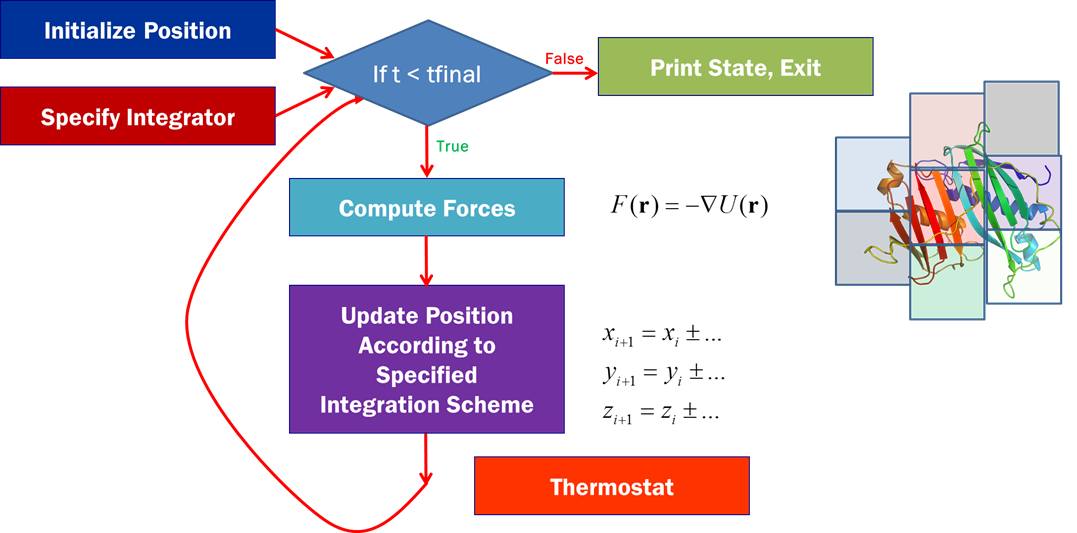
\includegraphics[width=0.85\textwidth]{mdfigure.png}
\caption{Molecular Dynamics algorithm graphical overview. MD begins with a system of particles coordinates and velocities, and integrates Newton's equation of motion forward in time utilizing a specified algorithm. A thermostat can be used to control the temperature through physics-based relationships between velocities and temperature. In this work, we implement the Nos\'{e}-Hoover Thermostat to control temperature.}
\label{fig:mdfigure}
\end{figure}

Several molecular dynamics packages exist to perform parallelized atomistic molecular dynamics simulations on CPUs.
%
These include LAMMPS \cite{Plimpton1995}, AMBER \cite{Case2010}, CHARMM \cite{MacKerell1998}, GROMACS \cite{Scott1999}, and TINKER \cite{Ponder2003}.
%
Only very recently, some of these packages have been updated in order to be implemented on Graphics Processing Units (GPUs) \cite{Brown2012,Brown2011,Gotz2012,Salomon-Ferrer2013}, and new packages exclusive to GPUs such as HOOMD-Blue\cite{Anderson2008} have been developed. %
The newly updated codes have not been nearly as extensively tested as their native CPU codebases, but can potentially offer significant speedups \url{http://ambermd.org/gpus/}.

Therefore, in this APC523 Final Project we built a new software package from scratch to run molecular dynamics simulations in parallel on both CPUs and GPUs. The GPU implementation is an ambitious goal very much working on the cutting-edge of computational science since few and only recent implementations exist on GPUs \cite{Anderson2008,Brown2012,Brown2011,Gotz2012,Salomon-Ferrer2013}.
%
The GPU implementation offers the promise of a significant speedup over CPU-only implementations.
%
The software implements the Lennard-Jones potential for interatomic interactions, a velocity-Verlet integrator, and a Nos\'{e}-Hoover thermostat. The developed software is sufficiently modular that other integration algorithms and pair potentials can easily be incorporated in future versions.
%
We chose to include the Lennard-Jones potential because many of the standard force fields \cite{Case2010,MacKerell1998,Scott1999,Kaminski2001,Arnautova2006,Khoury2013} today are built on Lennard-Jones interactions.
%
For example, a commonly used model for water, the TIP3P water model \cite{Jorgensen1983}, is composed of Lennard-Jones interactions and an additional electrostatic term to account for water's ability to be polarized.
%
In addition, Lennard-Jones particles serve as a very good model for monotomic gases such as argon \cite{Rahman1964} and condensed amorphous phases such as glasses \cite{Debenedetti2001}.

Because parallelization is essential for modern day molecular dynamics software, we implemented our software to run in parallel on both CPUs (with shared memory) and GPUs.
%
Our code is therefore fairly flexible and applicable to many different hardware architectures.

\section{Theory and Algorithms}

In the following section, we describe the theory and algorithms that underly the software developed.
%
In what follows, we assume that our system of interest consists of $N$ particles.
%
We denote the position, velocity, and acceleration of particle $i$ as $\mathbf{r}_i$, $\mathbf{v}_i$, and $\mathbf{a}_i$, respectively.
%
We denote the force on particle $i$ as $\mathbf{F}_i$.

In general, the algorithm for a molecular dynamics simulation is as follows (See Figure~\ref{fig:mdfigure}):
\begin{enumerate}
\item Initialize particle positions $\mathbf{r}_i$ and velocities $\mathbf{v}_i$ within the simulation box.
\item  \label{itm:MD_start} Calculate the forces $\mathbf{F}_i$ on each particle.
\item \label{itm:MD_end} Integrate forward the positions and velocities of each particle for the chosen timestep $\Delta t$.
\item Repeat steps \ref{itm:MD_start}-\ref{itm:MD_end} for the chosen amount of simulation time.
\end{enumerate}

% Here we show overall figure.
\subsection{Integrator} \label{subsec:integrator}

We implemented a velocity-Verlet integration algorithm \cite{Swope1982}, which is accurate to fourth order.
%
For a fixed number of particles (N), volume of the system (V), and energy (E), we update the positions and velocities of each atom using the following equations
\begin{eqnarray}
\mathbf{r}_i (t + \Delta t)  & = & \mathbf{r}_i(t) + \mathbf{v}_i(t) \Delta t + \mathbf{a}_i(t) \frac{\Delta t^2}{2} \\
\mathbf{v}_i(t + \Delta t) & = & \mathbf{v}_i(t) + \left[\mathbf{a}_i(t) + \mathbf{a}_i(t + \Delta t) \right] \frac{\Delta t}{2}
\end{eqnarray}
where $\mathbf{a}_i = \mathbf{F}_i/m$.
%
The forces can be calculated from the potential energy function and will be discussed further in subsection \ref{subsec:potential}.

Because $\mathbf{v}_i$ depends on both $\mathbf{a}_i(t)$ and $\mathbf{a}_i(t+\Delta t)$, the order of computations goes as follows
\begin{enumerate}
\item Calculate $\mathbf{r}_i(t + \Delta t)$ from $\mathbf{r}_i(t)$, $\mathbf{v}_i(t)$, and $\mathbf{a}_i(t)$.
\item Calculate $\mathbf{a}_i(t + \Delta t)$ from $\mathbf{r}_i(t + \Delta t)$.
\item Calculate $\mathbf{v}_i(t + \Delta t)$ from $\mathbf{v}_i(t)$, $\mathbf{a}_i(t)$, and $\mathbf{a}_i(t + \Delta t)$.
\end{enumerate}

\subsection{Thermostats} \label{subsec:thermostat}
The equations in \ref{subsec:integrator} are only for NVE simulations.
%
If we are instead interested in fixing temperature (T) rather than energy (E), we must introduce the idea of a {\em thermostat} to our simulations.
%
A thermostat is necessary in most simulations since experiments are not typically done at constant energy.
%
The thermostat adjusts the velocities of the particles so that they (on average) maintain a user-specified desired temperature.

We implemented a time-reversible Nos\'{e}-Hoover thermostat in our molecular dynamics software.
%
The Nos\'{e}-Hoover thermostat adjusts the particle velocities based on the target temperature of the system and the current kinetic energy of the system.
%
The thermostat is governed by its own equation of motion given by the position ($\xi$), velocity ($\dot{\xi}$), and acceleration ($\ddot{\xi}$) of the thermostat.

Let $T_{set}$ be the desired temperature.
%
Then the acceleration of the thermostat is given by
\begin{equation}
\ddot{\xi} = \frac{1}{Q} \left[ \sum_{i=1}^{N} m_i v_i^2 - N_f k_B T_{set} \right]
\end{equation}

The equations of motion for the particles and the thermostat are
\begin{eqnarray}
r_i(t + \Delta t) &=& r_i(t) + v_i(t) \Delta t + \left[ a_i(t) - v_i(t)\dot{\xi}(t) \right] \frac{\Delta t^2}{2}\\
v_i(t + \Delta t) &=& v_i(t) + \left[ a_i(t) - v_i(t) \dot{\xi}(t) \right] \frac{\Delta t}{2} + \left[a_i(t + \Delta t)  - v_i(t + \Delta t) \dot{\xi}(t + \Delta t) \right] \frac{\Delta t}{2} \\
\xi(t + \Delta t) & = & \xi(t) + \dot{\xi}(t) \Delta t + \ddot{\xi}(t) \frac{\Delta t^2 }{2} \\
\dot{\xi}(t + \Delta t)  & = & \dot{\xi}(t) + \left[ \ddot{\xi}(t) + \ddot{\xi} (t + \Delta t)  \right] \frac{\Delta t}{2}
\end{eqnarray}

The Nos\'{e}-Hoover thermostat can be shown to be time-reversible when it is implemented via the following algorithm.
First, update the thermostat velocity using a half-step in time
\begin{equation}
\dot{\xi} (t+ \Delta t/2) = \dot{\xi}(t) + \ddot{\xi}(t) \frac{\Delta t}{2}
\end{equation}
and thermostat position.
\begin{equation}
\xi (t+ \Delta t) = \xi(t) + \dot{\xi}(t+\Delta t/2)\Delta t
\end{equation}
Second, evolve the particle velocities with a half-step.
\begin{equation}
v_i (t+\Delta t/2) = v_i (t) \exp^{-\dot{\xi}(t+\Delta t/2) \Delta t/2} + a_{i} (t) \Delta t/2
\end{equation}
Third, evolve particle positions.
\begin{equation}
r_{i} (t+\Delta t) + r_{i} (t) + v_{i}(t+ \Delta t/2) \Delta t
\end{equation}
Fourth, call the function \textbf{calcForce} to update the accelerations at the next timestep.
\begin{equation}
a_{i} (t+\Delta t) = F_{i} (t+ \Delta t)/m_{i}
\end{equation}
Fifth, evolve the particle velocities.
\begin{equation}
v_{i} (t+ \Delta t)  = [v_{i}(t+\Delta t/2) + a_{i}(t+\Delta t) \Delta t/2]\exp^{-\dot{\xi}(t+\Delta t/2) \Delta t/2}
\end{equation}
Finally, the thermostat velocity is updated.
\begin{equation}
\dot{\xi}(t+\Delta t) = \dot{\xi} (t+\Delta t/2) + \ddot{\xi} (t+\Delta t) \Delta t /2
\end{equation}
The thermostat acceleration, $\ddot{\eta}(t)$ is expressed in the form
\begin{equation}
\ddot{\xi}(t) = \frac{1}{\tau^{2}} [\frac{T(t)}{T_{target}} -1 ]
\end{equation}
where $\tau^{2} = \frac{Q}{(3N-1)*T_{target}}$ and $Q$, which is the thermal mass of the thermostat spring equal to unity.
Because this algorithm is time-reversible, this algorithm is implemented in our software.
% END OF THAT DOC.

This is an algorithmic advance discovered 20 years ago.
The three factors in G are separate and unitary, therefore. This means that any integrator  based on this Trotter factorization will be time-reversible. CITE Reversible multiple time scale molecular dynamics by Tuckermar Berne Martyna

\subsection{Pair potentials} \label{subsec:potential}

We implemented a shifted Lennard-Jones pair potential in our molecular dynamics software.
%
In the shifted Lennard-Jones potential, the potential energy of interaction between two particles is a function of the interatomic distance $r = \|\mathbf{r}_i - \mathbf{r}_j \|$, and is given by
\begin{equation}
U(r) = 4 \epsilon\left[ \left( \frac{\sigma}{r-\delta} \right)^{12} - \left( \frac{\sigma}{r-\delta} \right)^6 \right] + U_{shift}
\end{equation}
where $\epsilon$, $\sigma$, $\delta$, and $U_{shift}$ are adjustable parameters.
%
The total potential energy of the system is then given by
\begin{equation}
U_{tot} = \sum_{i=1}^{N} \sum_{j=1}^{i-1} U\left( \| r_i - r_j \| \right)
\end{equation}

The force on a particle $F_i$ is the gradient of the potential, $F_i = \nabla_i U_{tot}$.
%
It can be shown that
\begin{equation}
F_{i, x} = \sum_{j \ne i} \frac{d U\left( \| r_i - r_j \| \right)}{d \| r_i - r_j \| } \frac{x_i - x_j}{\|r_i - r_j\|}.
\end{equation}

The potential energy and force calculations involve $\mathcal{O}(N^2)$ calculations, since each of the $N$ particles interacts with the remaining $N-1$ particles.
%
Therefore, the potential energy and force calculation are the portions that are typically parallelized in an MD code.

\subsection{Parallelization}

We implemented parallelization on CPUs and GPUs in our molecular dynamics software.
%
On CPUs, we parallelized our code using OpenMP and therefore, our code can run in parallel on any shared memory cluster.
%
On GPUs, we parallelized our code using CUDA.
The parallelization on GPUs is implemented in the force calculation, which accounts for XXXXX percent of the cost of the simulation according to our profiling studies.
%
Parallelization and scaling was tested on the Adroit and TIGER clusters.
\subsection{Neighbor lists}

\subsection{Testing}

We implemented Google Tests within our software.

% What are the tests ?!??!

\section{Code Structure and Implementation Notes}

The software is implemented in C++ and version-controlled through an actively updated github repository \url{https://github.com/PrincetonUniversity/CBEMDGPU}.
%
The class structure is as follows
\begin{description}

\item[\texttt{common.h}] This class implements the error catching functions.

\item[\texttt{cudaHelper.h}] This function implements the cuda code for paralleization on GPUs.

\item[\texttt{cellList.cpp}] This class controls the cell lists (for parallelization on CPU) or neighbor lists (for parallelization on GPUs).

\item[\texttt{dataTypes.h}] This function implements the custom structures, such as the atom struct, which stores the position, velocity, and acceleration of an atom.
	
\item[\texttt{integrator.cpp}] This class is a ``virtual'' class (maybe????)

\item[\texttt{nve.cpp}] This class implements the velocity-Verlet integration scheme for an NVE simulation.

\item[\texttt{nvt.cpp}] This class implements the velocity-Verlet integration scheme with a Nos\'{e}-Hoover thermostat for an NVT simulation.

\item[\texttt{potential.cpp}] The potential class implements the force and potential energy calculations for the standard Lennard-Jones potential.
%
This class can be expanded to include other potential energy functions.

\item[\texttt{system.cpp}] This class stores all of the parameters relevant to the simulation system, such as the box size, potential energy function, and the number of atoms.

\item[\texttt{utils.cpp}] This class implements the necessary ``helper'' functions for the simulation, such as the distance calculation with periodic boundary conditions using the minimum image convention.

\item[\texttt{main.cpp}]

\item[\texttt{unittests.cpp}]

\end{description}
\section{Results}

\subsection{Scaling studies}

We should discuss the fact that we performed optimizations while we were coding this.

\subsection{Benchmarking}

\subsection{Validation against literature values}

MSD
g(r)
Temp and Energy consistencies.
\subsection{Image from VMD}
We should attach an image from MD for a system of particles and we should also attach a small MD movie as a file viewable in Windows from an .xyz file for them to view and we should note that here.
\section{Conclusions and Future Work}

\pagebreak
\bibliographystyle{proteins1}
\bibliography{references}

\end{document}
